\documentclass[11pt]{article}

% This must be in the first 5 lines to tell arXiv to use pdfLaTeX, which is strongly recommended.
\pdfoutput=1
% In particular, the hyperref package requires pdfLaTeX in order to break URLs across lines.

% Change "review" to "final" to generate the final (sometimes called camera-ready) version.
% Change to "preprint" to generate a non-anonymous version with page numbers.
\usepackage[preprint]{acl}

% Standard package includes
\usepackage{times}
\usepackage{latexsym}

% For proper rendering and hyphenation of words containing Latin characters (including in bib files)
\usepackage[T1]{fontenc}
% For Vietnamese characters
% \usepackage[T5]{fontenc}
% See https://www.latex-project.org/help/documentation/encguide.pdf for other character sets

% This assumes your files are encoded as UTF8
\usepackage[utf8]{inputenc}

% This is not strictly necessary, and may be commented out,
% but it will improve the layout of the manuscript,
% and will typically save some space.
\usepackage{microtype}

% This is also not strictly necessary, and may be commented out.
% However, it will improve the aesthetics of text in
% the typewriter font.
\usepackage{inconsolata}

%Including images in your LaTeX document requires adding
%additional package(s)
\usepackage{graphicx}

\usepackage[utf8]{inputenc} % allow utf-8 input
\usepackage[T1]{fontenc}    % use 8-bit T1 fonts
\usepackage{hyperref}       % hyperlinks
\usepackage{url}            % simple URL typesetting
\usepackage{booktabs}       % professional-quality tables
\usepackage{amsfonts}       % blackboard math symbols
\usepackage{nicefrac}       % compact symbols for 1/2, etc.
\usepackage{microtype}      % microtypography
\usepackage{xcolor}         % colors
\usepackage{array}
\usepackage{amssymb}
\usepackage{enumitem}
\usepackage{graphicx}
\usepackage{subcaption}
\usepackage{threeparttable}
\usepackage{pifont}
\usepackage{amsmath}
\usepackage{multirow}
\newcommand{\xmark}{\ding{55}}
\usepackage{listings}

% If the title and author information does not fit in the area allocated, uncomment the following
%
%\setlength\titlebox{<dim>}
%
% and set <dim> to something 5cm or larger.

\definecolor{red}{RGB}{238, 68, 51}
\definecolor{blue}{RGB}{70, 177, 225}
\definecolor{yellow}{RGB}{255, 192, 0}
\definecolor{purple}{RGB}{216, 110, 204}
\definecolor{brown}{RGB}{127, 36, 28}
\definecolor{green}{RGB}{71, 172, 20}
\definecolor{orange}{RGB}{194,153,107}

\newcommand{\cyx}[1]{{\color{brown}{#1}}}
\newcommand{\hsy}[1]{{\color{yellow}{#1}}}

% \newcommand{\cyx}[1]{{#1}}
\newcolumntype{C}[1]{>{\centering\let\newline\\\arraybackslash\hspace{0pt}}m{#1}}

\lstdefinestyle{prompt}{
    basicstyle=\ttfamily\small, % Use monospaced font
    backgroundcolor=\color{gray!10}, % Light gray background
    frame=single, % Single line border
    rulecolor=\color{black}, % Border color
    breaklines=true, % Allow line breaks
    captionpos=b % Caption at the bottom
}

\title{A3: Android Agent Arena for Mobile GUI Agents}

% Author information can be set in various styles:
% For several authors from the same institution:
% \author{Author 1 \and ... \and Author n \\
%         Address line \\ ... \\ Address line}
% if the names do not fit well on one line use
%         Author 1 \\ {\bf Author 2} \\ ... \\ {\bf Author n} \\
% For authors from different institutions:
% \author{Author 1 \\ Address line \\  ... \\ Address line
%         \And  ... \And
%         Author n \\ Address line \\ ... \\ Address line}
% To start a separate ``row'' of authors use \AND, as in
% \author{Author 1 \\ Address line \\  ... \\ Address line
%         \AND
%         Author 2 \\ Address line \\ ... \\ Address line \And
%         Author 3 \\ Address line \\ ... \\ Address line}

\author{Yuxiang Chai \\
  MMLab @ CUHK \\
  \And
  Hanhao Li \\
  EE department @ CUHK \\
  \And
  Jiayu Zhang \\
  EE department @ CUHK \\
  \AND
  Liang Liu \\
  vivo AI Lab \\
  \And
  Guangyi Liu \\
  vivo AI Lab \\
  \And
  Guozhi Wang \\
  vivo AI Lab \\
  \AND
  Shuai Ren \\
  vivo AI Lab \\
  \And
  Siyuan Huang \\
  Shanghai Jiao Tong University \\
  \And
  Hongsheng Li\thanks{Corresponding Author} \\
  MMLab @ CUHK }

% \author{
%  \textbf{Yuxiang Chai\textsuperscript{1}},
%  \textbf{Jiayu Zhang\textsuperscript{2}},
%  \textbf{Hanhao Li\textsuperscript{2}},
%  \\
%  \textbf{Siyuan Huang\textsuperscript{3}},
%  \textbf{Hongsheng Li\textsuperscript{1,4}},
% \\
%  \textsuperscript{1}MMLab @ CUHK,
%  \textsuperscript{2}EE department @ CUHK,
%  \textsuperscript{3}Shanghai Jiao Tong University,
% \\
%  \small{
%    \textbf{Correspondence:} \href{mailto:email@domain}{email@domain}
%  }
% }

\begin{document}
\maketitle
\begin{abstract}
AI agents have become increasingly prevalent in recent years, driven by significant advancements in the field of large language models (LLMs). Mobile GUI agents, a subset of AI agents, are designed to autonomously perform tasks on mobile devices. While numerous studies have introduced agents, datasets, and benchmarks to advance mobile GUI agent research, many existing datasets focus on static frame evaluations and fail to provide a comprehensive platform for assessing performance on real-world, in-the-wild tasks. To address this gap, we present Android Agent Arena (A3), a novel evaluation platform. Unlike existing in-the-wild systems, A3 offers: (1) meaningful and practical tasks, including real-time online information retrieval and operational instructions; (2) a larger, more flexible action space, enabling compatibility with agents trained on any dataset; and (3) automated commercial LLM-based evaluation process which supports task customization. A3 includes 20 widely used general third-party apps and 201 tasks representative of common user scenarios, providing a robust foundation for evaluating mobile GUI agents in real-world situations and a new autonomous evaluation process for less human labor and coding expertise.
\end{abstract}


\begin{figure*}
    \centering
    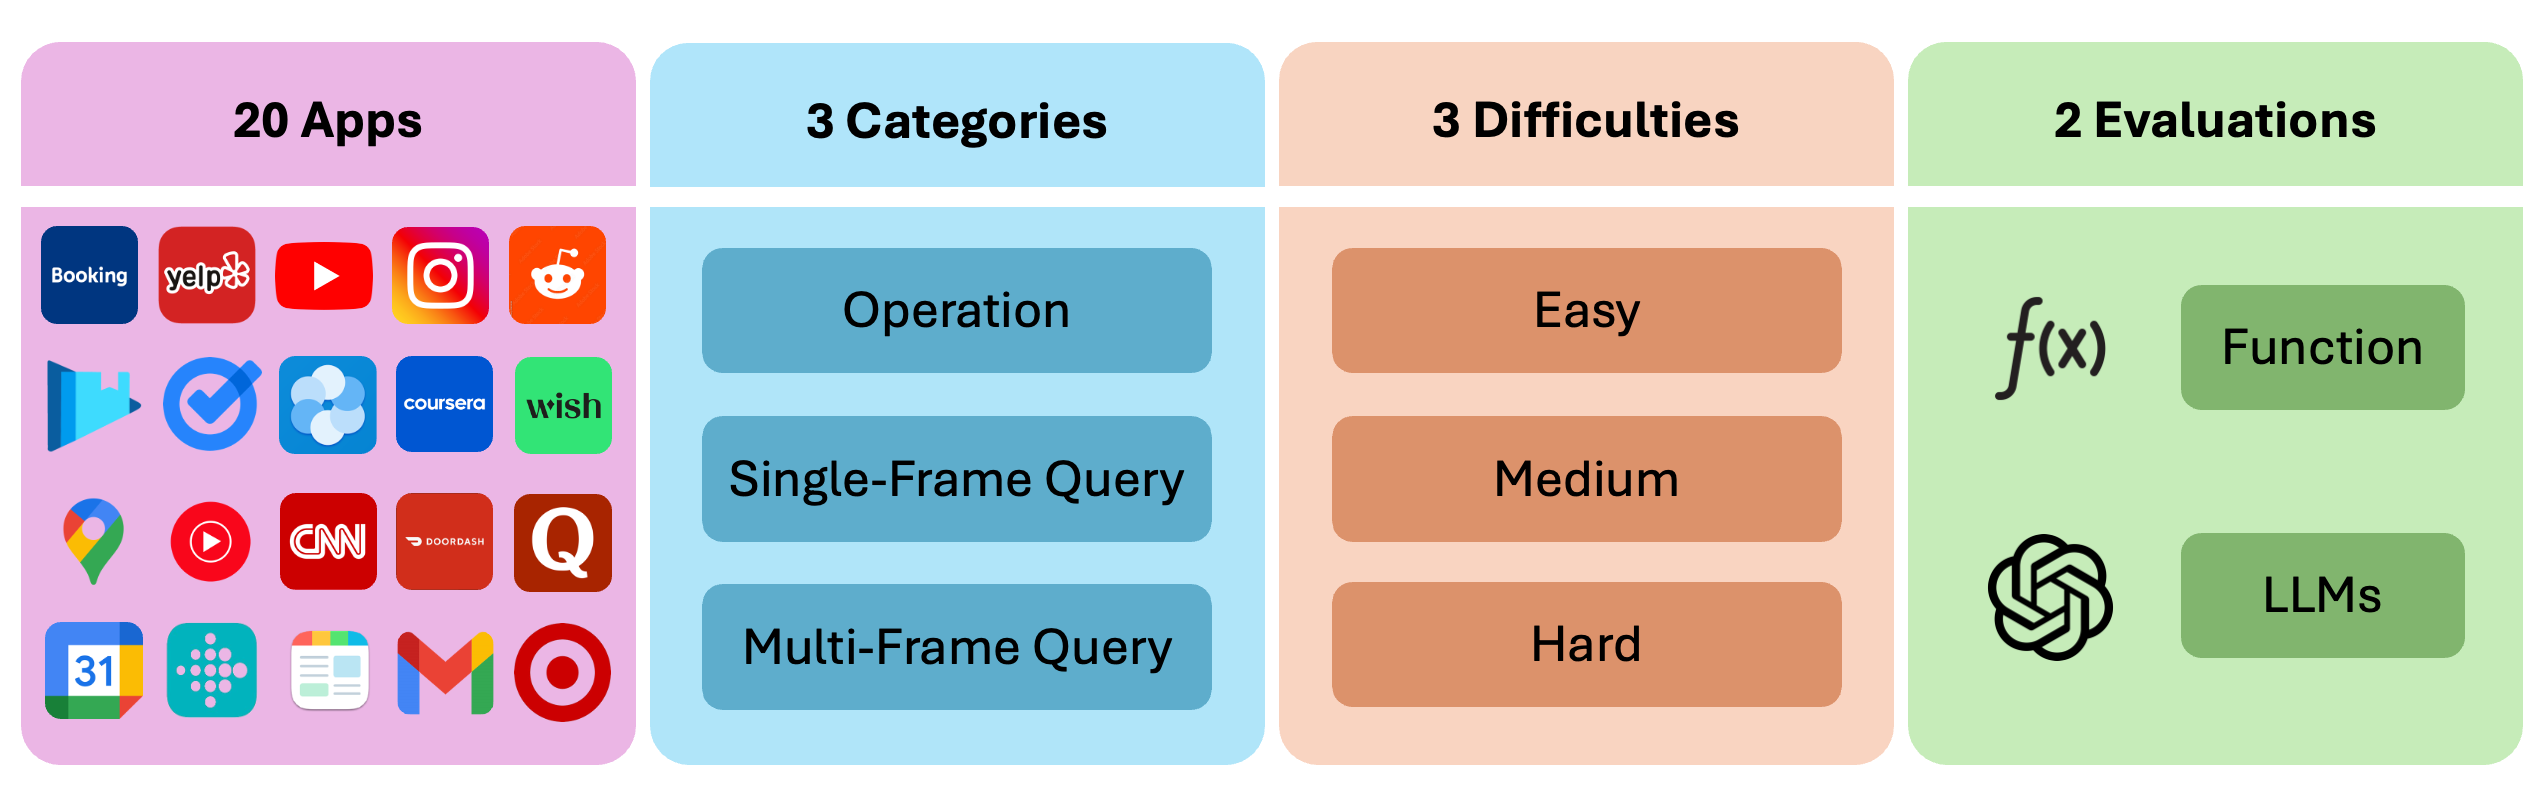
\includegraphics[width=0.96\linewidth]{images/overview.png}
    \caption{Overview of Android Agent Arena. A3 contains 201 tasks from 20 widely used apps. Tasks are categorized into operation, single-frame query and multi-frame query based on the task goal. Tasks are also split into three difficulty levels based on the human operation steps. A3 also integrates two evaluation methods for different use cases.}
    \label{fig:overview}
\end{figure*}



\section{Introduction}


Existing mobile AI assistants such as Siri, Xiao AI, and Bixby have demonstrated the potential of mobile agents to facilitate interactions between human users and mobile devices. However, those assistants are only effective in managing the routine tasks such as reporting weather condition and performing web searches due to the nature that they use APIs to perform task automation. To broaden the capability of AI agents, researchers have proposed GUI agents~\citep{liu2025llm}, which leverage the extended world knowledge and robust capabilities of multimodal large language models (MLLM) to effectively complete tasks on third-party general apps without the reliance on the APIs. 


Despite the promising advancements in GUI agents, the majority of existing GUI-control datasets~\citep{rawles2024androidinthewild, chai2024amex, li2024androidcontrol} and primarily focus on static frame evaluations, which have significant limitations. These datasets typically provide a collection of screenshots or UI states, requiring agents to predict the next action based on a single, frozen frame. Such an approach fails to capture the dynamic and interactive nature of real-world mobile tasks, where agents must navigate through sequences of actions, adapt to changing app states, and handle unexpected outcomes. Furthermore, static frame evaluations often lack contextual information about task flows, making it difficult to assess an agent’s ability to perform multi-step or goal-oriented tasks. This disconnect between static frame evaluations and real-world usage scenarios results in a gap between the capabilities of current GUI agents and the demands of practical applications, underscoring the need for a more comprehensive and interactive evaluation platform.

Several recent works~\citep{rawles2024androidworld, xing2024androidarena, xu2024androidlab, lee2024bmoca, zhang2023mobileenv} have introduced dynamic evaluation platforms for Android GUI agents. While these efforts represent significant progress, they suffer from critical limitations that hinder their effectiveness as comprehensive evaluation benchmarks. For instance, many platforms restrict app selection to Google apps, F-Droid apps (non-mainstream open-source apps), or static offline apps, which do not reflect the diversity or complexity of real-world usage. Additionally, these platforms often provide only a limited diversity of tasks and do not support task customization, or fail to include information query tasks, which are essential for evaluating practical agent performance. To address these shortcomings, we propose \textbf{Android Agent Arena} (A3), a novel evaluation system that offers: (i) integration with 20 widely used third-party apps and 201 tasks designed around real-world app functionalities, (ii) a diverse set of tasks categorized into three distinct types, and (iii) a larger action space, enabling compatibility with agents trained on any dataset. Furthermore, we introduce a new evaluation method that leverages the capabilities of commercial LLMs to automate task evaluation, significantly reducing the need for human intervention and manual coding. Table~\ref{fig:overview} demonstrates the overview of A3.

Our contributions can be summarized as follows:
\begin{itemize}[leftmargin=5mm]
\item We introduce Android Agent Arena (A3), a comprehensive evaluation platform that integrates 201 diverse multi-category tasks across 20 mainstream apps from real-world scenarios, with support for an expanded action space compatible with any dataset annotation style. 
\item We propose a novel evaluation approach leveraging commercial LLMs, which enables scalable and automated evaluation processes while greatly reducing the need for manual effort in task evaluation and keeping the evaluation precision, suitable for customized tasks evaluation.
\end{itemize}



\begin{table*}
    \centering
    \begin{tabular}{l c c c c c c}
        \toprule
        Name & Eval Mode & \# Tasks  & \# General Apps & Operation & Inf. Query & Online \\
        \midrule
        \textsc{AitW} & static & -  & - & \checkmark & \xmark & \xmark \\
        \textsc{AndroidControl} & static  & - & - & \checkmark & \xmark & \xmark \\
        \textsc{AMEX} & static & -  & - & \checkmark & \xmark & \xmark \\
        \midrule

        AndroidArena & dynamic & 221  & 4 & \checkmark & \xmark & \checkmark\\
        Mobile-Env & dynamic & 74  & 5 & \checkmark & \xmark & \checkmark \\
        AndroidWorld & dynamic & 116  & 15 & \checkmark & \xmark & \checkmark\\
        B-Moca & dynamic & 131 & 4  & \checkmark & \xmark & \checkmark \\
        AndroidLab & dynamic & 138  & 5 & \checkmark & \checkmark & \xmark \\
        \midrule

        A3 (Our) & dynamic & 201  & 20 & \checkmark & \checkmark & \checkmark\\
        \bottomrule
    \end{tabular}
    \caption{GUI related datasets and benchmarks. The top three rows are GUI-related datasets, which provide static frame evaluation. The middle five rows are dynamic evaluation systems, which provide different tasks from different apps in different settings. AndroidWorld provides 15 generals apps from non-mainstream open-source F-Droid.}
    \label{tab:compare-benchmark}
\end{table*}





\section{Related Work}

\subsection{GUI Agent}

Recent advancements have begun leveraging the extensive world knowledge and robust reasoning capabilities of LLMs~\citep{gu2024mamba, gur-etal-2023-understanding, touvron2023llama} for task planning and execution. A notable approach involves using general-purpose business-level models, such as GPT-4v, as GUI-control agents. Studies like~\citep{yang2023appagent, pmlr-v235-zheng24e} employ extensive prompt engineering to guide these models in performing complex tasks. An alternative research direction focuses on fine-tuning smaller LLMs using GUI-specific datasets to imbue them with domain-specific knowledge, thereby improving their efficiency and task performance. For instance, CogAgent~\citep{hong2024cogagent} enhances GUI task performance by incorporating a high-resolution cross-module that fuses image features at multiple levels. SphAgent~\citep{chai2024amex} utilizes the element functionalities to further enhance the screen and element understanding. UI-TARS~\citep{qin2025ui-tars} finetunes the model with more reasoning data and GUI perception data. Qwen2.5-VL is a generalist Multimodal Large Language Model (MLLM) which pretrains on GUI-related data and achieved sound performance on various benchmarks.

\subsection{GUI-related Dataset}

The introduction of the Rico dataset series~\citep{Deka:2017:Rico, sunkara-etal-2022-towards} marked a significant milestone in GUI-related research by providing foundational datasets for GUI element classification and detection. Subsequent works~\citep{burns2021motif, gubbi-venkatesh-etal-2024-ugif} introduced small-scale, instruction-based GUI control datasets. Among these, UGIF~\citep{gubbi-venkatesh-etal-2024-ugif} stands out as a multilingual dataset supporting eight languages. \textsc{AitW}\citep{rawles2024androidinthewild} expanded the field with a large-scale dataset, but it suffered from significant redundancy in instructions and frequent mis-annotations. To address this, \textsc{AitZ}\citep{zhang-etal-2024-aitz} refined \textsc{AitW} by applying Chain-of-Action-Thought re-annotation, resulting in a cleaner but much smaller dataset. \textsc{AndroidControl}\citep{li2024androidcontrol} further introduced a large-scale dataset, albeit with simpler tasks and a distinct action space compared to \textsc{AitW} and \textsc{AitZ}. Meanwhile, AMEX\citep{chai2024amex} redefined GUI element annotation by incorporating element functionality, enabling agents to better interpret mobile GUI designs, and pushed the boundaries with more complex tasks than prior datasets. However, despite their contributions, these datasets are limited to static frame evaluations, where agents predict actions based on a single screenshot, an instruction, and a ground-truth history of actions. This approach fails to capture the dynamic and interactive nature of real-world scenarios, where historical actions are unavailable, and a single error can cascade and severely impact subsequent performance. This highlights the need for evaluation systems that better reflect the complexities of real-world task execution.

\subsection{Dynamic Evaluation Benchmark}

To overcome the limitations of static frame evaluations, researchers have developed several dynamic evaluation systems~\citep{lee2024bmoca, xu2024androidlab, xing2024androidarena, rawles2024androidworld, zhang2023mobileenv} that aim to better simulate real-world environments (See Table~\ref{tab:compare-benchmark}). However, these systems still suffer from several shortcomings that limit their applicability and realism. For instance, Mobile-Env~\citep{zhang2023mobileenv} is restricted to only 74 tasks, limiting its comprehensiveness of task diversity. AndroidArena~\citep{xing2024androidarena} expands the task set by including cross-app interactions, yet it is restricted to Google apps and built-in system apps (e.g., settings and clock), which are already manageable by API-based assistants, thus failing to assess general usability across diverse third-party applications. B-Moca~\citep{lee2024bmoca} introduces a Korean language setting, but its tasks are overly simplistic and lack diversity, making it inadequate for evaluating complex interactions (e.g., ``input 1 in Calculator'', ``go to account tab in Walmart''). AndroidWorld~\citep{rawles2024androidworld} attempts to introduce variety by utilizing open-source apps from F-Droid\footnote{https://f-droid.org/en/packages/}. However, these apps often differ significantly from mainstream app designs, making them unrepresentative of real-world usage scenarios. A critical limitation across all these systems is their narrow focus on operational instructions and corresponding evaluations, neglecting more complex real-world interactions. AndroidLab~\citep{xu2024androidlab} makes an important step forward by incorporating information query instructions and evaluations, but it remains constrained by its reliance on offline and static apps. This limitation excludes crucial categories such as news, shopping, email, and music, which are integral to real-world user experiences. Additionally, the evaluation methodologies used in existing systems are often simplistic, primarily relying on element matching~\citep{lee2024bmoca} or predefined answers~\citep{xu2024androidlab}, which fail to capture the nuances of naturalistic interactions and adaptive responses. Furthermore, all existing systems do not provide a solution for customized tasks evaluation, which is important for other common tasks not covered in the systems.

\begin{figure*}
    \centering
    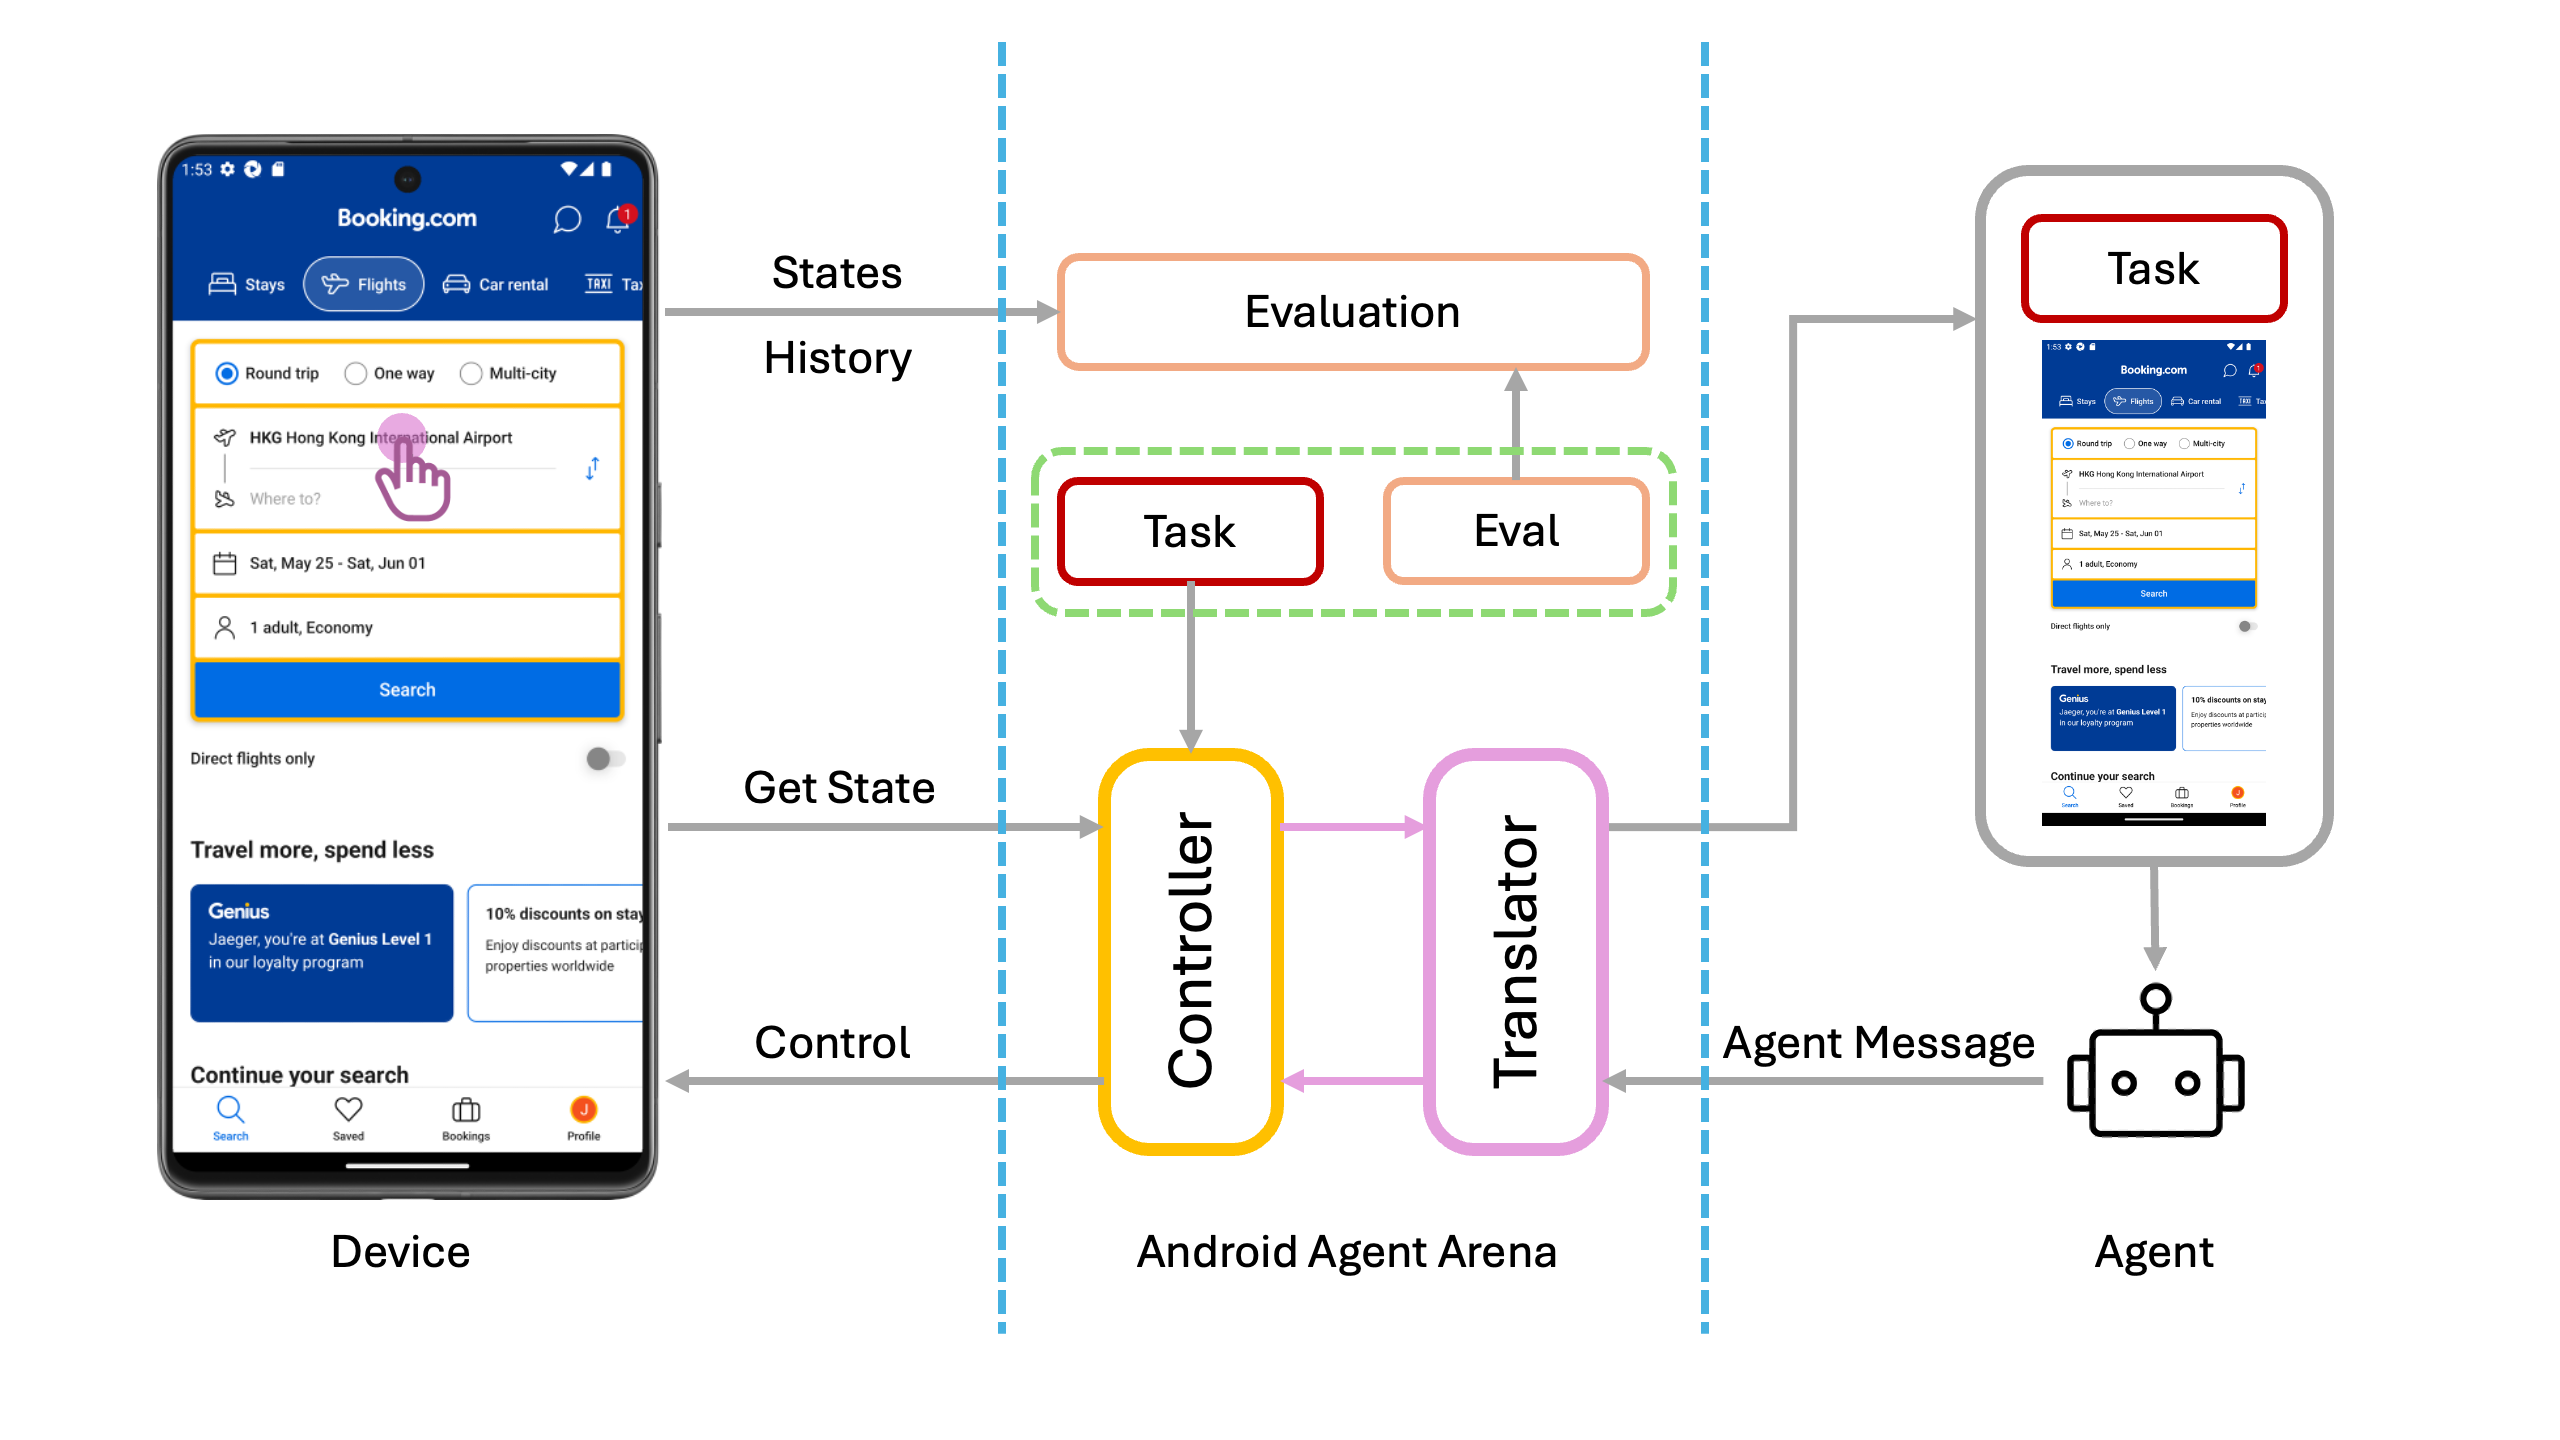
\includegraphics[width=0.9\linewidth]{images/pipeline.png}
    \caption{Overview of Android Agent Arena. A3 contains controller, evaluator, and translator. The controller is responsible for controlling and getting the state of the device. The translator is responsible for translating the device function and the agent messages. The evaluator is responsible for the final evaluation.}
    \label{fig:pipeline}
\end{figure*}

\section{Android Agent Arena (A3)}

\subsection{Overview}

A3 is a lightweight system built on Appium\footnote{https://appium.io/docs/en/latest/}, an open-source framework for controlling Android and iOS devices. As shown in Figure~\ref{fig:pipeline}, A3 acts as a bridge between a GUI agent and an Android device. It integrates tasks with their corresponding evaluation functions. The process begins with the controller retrieving the device's current state, which includes a screenshot and an Extensible Markup Language (XML) file. This state and task instruction, along with additional information such as previous screenshots, XML files, and actions, is then sent to the agent. The agent analyzes the input and predicts the next action to take based on the current state. The predicted action is passed to the translator, which converts it into device control commands to interact with the device. This loop continues until the agent signals task completion or the predefined maximum number of steps is reached. For evaluation process, users can choose from function evaluation and commercial LLM evaluation, based on their needs and budgets. A3 also provides optional essential states evaluation for commercial LLM evaluation method to fully assess the ability of agents. The details of app selection and task generation is in Appendix~\ref{app:app-selection} and ~\ref{app:task-gen-eg}.

\subsection{Action Space}

\textsc{AitW}, \textsc{AitZ}, and AMEX share the same action space: {\texttt{CLICK}, \texttt{SCROLL}, \texttt{TYPE}, \texttt{ENTER}, \texttt{BACK}, \texttt{HOME}, \texttt{COMPLETE}, \texttt{IMPOSSIBLE}}. In contrast, \textsc{AndroidControl} introduces a different action space that includes two additional actions: \texttt{Open}, \texttt{Long Press} and \texttt{WAIT}. The \texttt{Open} action is specifically defined to directly launch an app and the \texttt{WAIT} action means the current state is still loading and needs to wait. However, no existing evaluation system currently supports these additional actions, making it impossible to test agents trained on \textsc{AndroidControl}. To address this limitation, we extend A3 to accommodate a larger action space, which contains all the action types of all datasets, ensuring compatibility with agents trained on any dataset.

\begin{table}[t]
    \centering
    % \begin{tabular}{l c}
    % \toprule
    %     Split & Number \\
    %     \midrule
    %     Easy & 94 \\
    %     Medium & 77 \\
    %     Hard & 30 \\
    %     \midrule
    %     Operation & 143 \\
    %     Single Query & 49 \\
    %     Multi Query & 9 \\
    % \bottomrule
    % \end{tabular}
    \begin{tabular}{c c c | c c c}
        \toprule
        Easy & Med. & Hard & Op. & S.Q & M.Q \\
        \midrule
        94 & 77 & 30 & 143 & 49 & 9 \\
        \bottomrule
    \end{tabular}
    \caption{The distribution of tasks in A3. ``Op'' stands for operation. ``S.Q.'' and ``M.Q'' stands for single-page query and multi-page query respectively. }
    \label{tab:distribution}
\end{table}

\subsection{Task}

% \begin{figure}
%     \centering
%     \begin{subfigure}{1\linewidth}
%         \centering
%         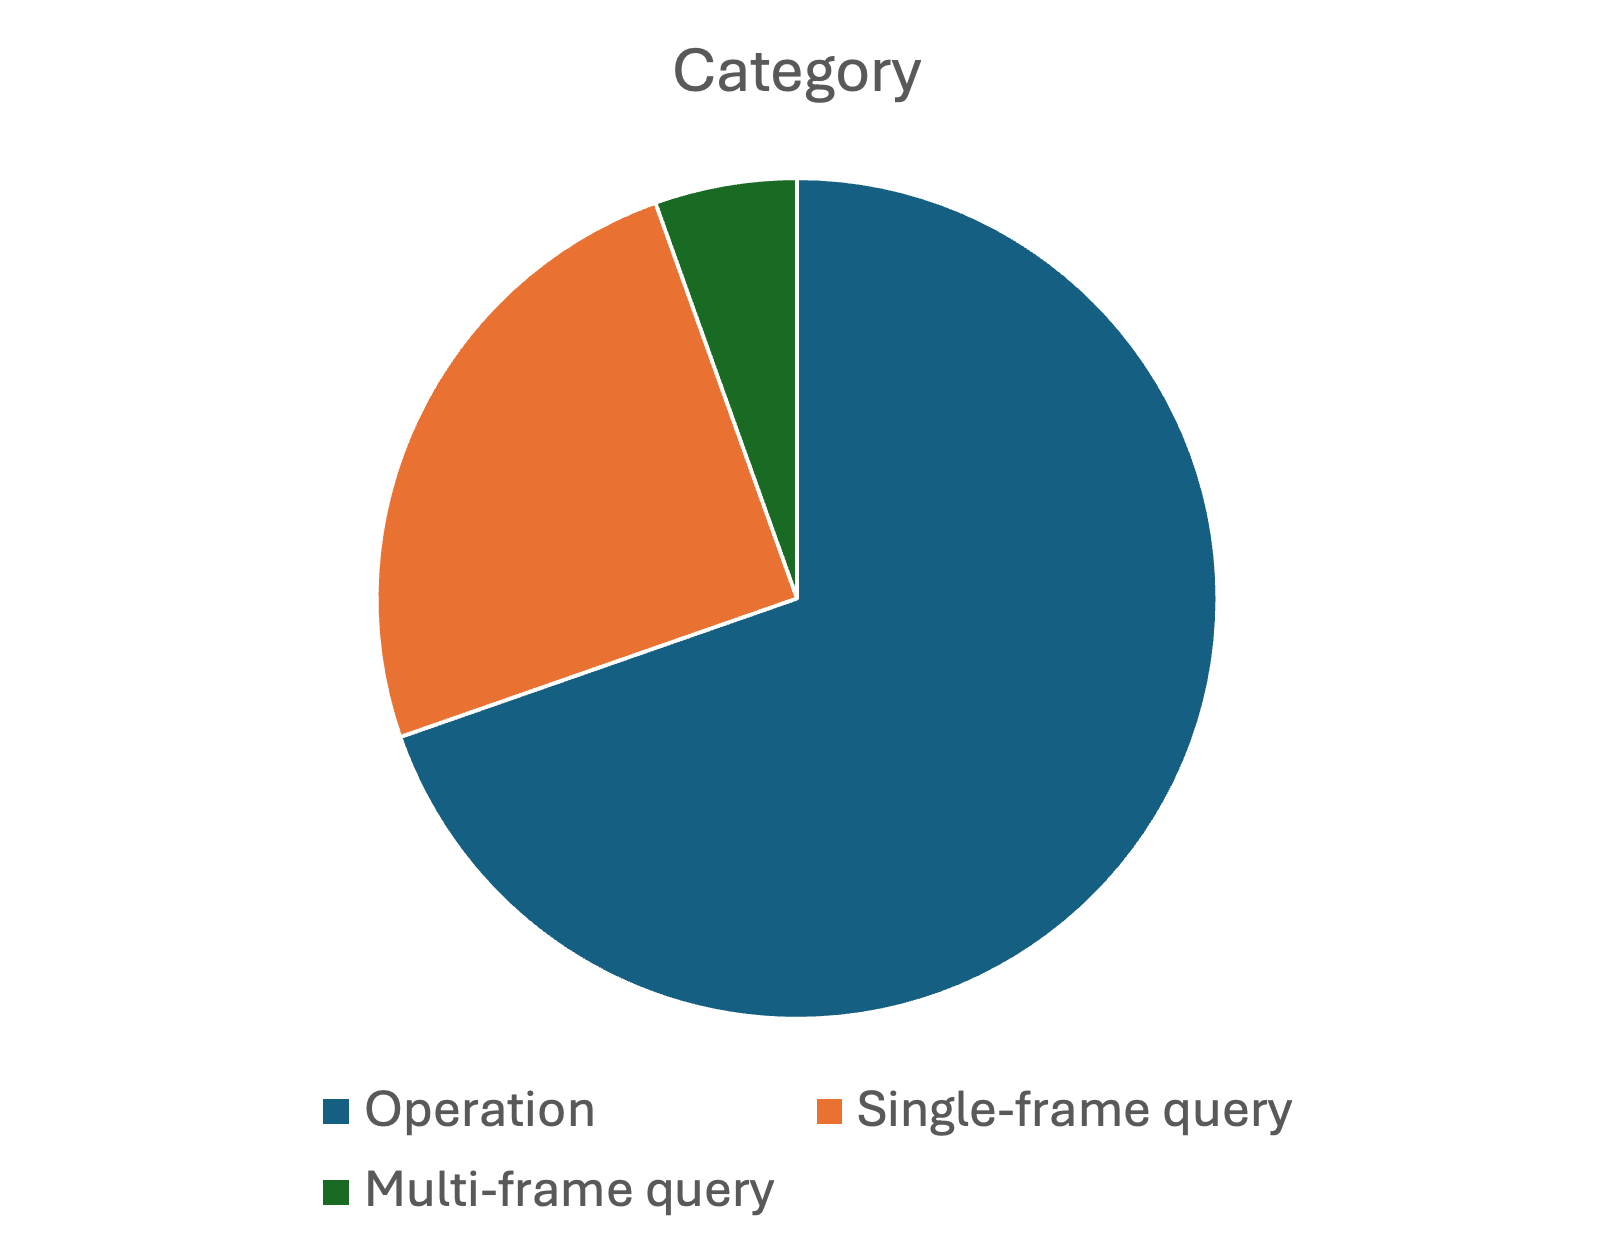
\includegraphics[width=0.8\textwidth]{images/dist_category.png}
%     \end{subfigure}
%     \begin{subfigure}{1\linewidth}
%         \centering
%         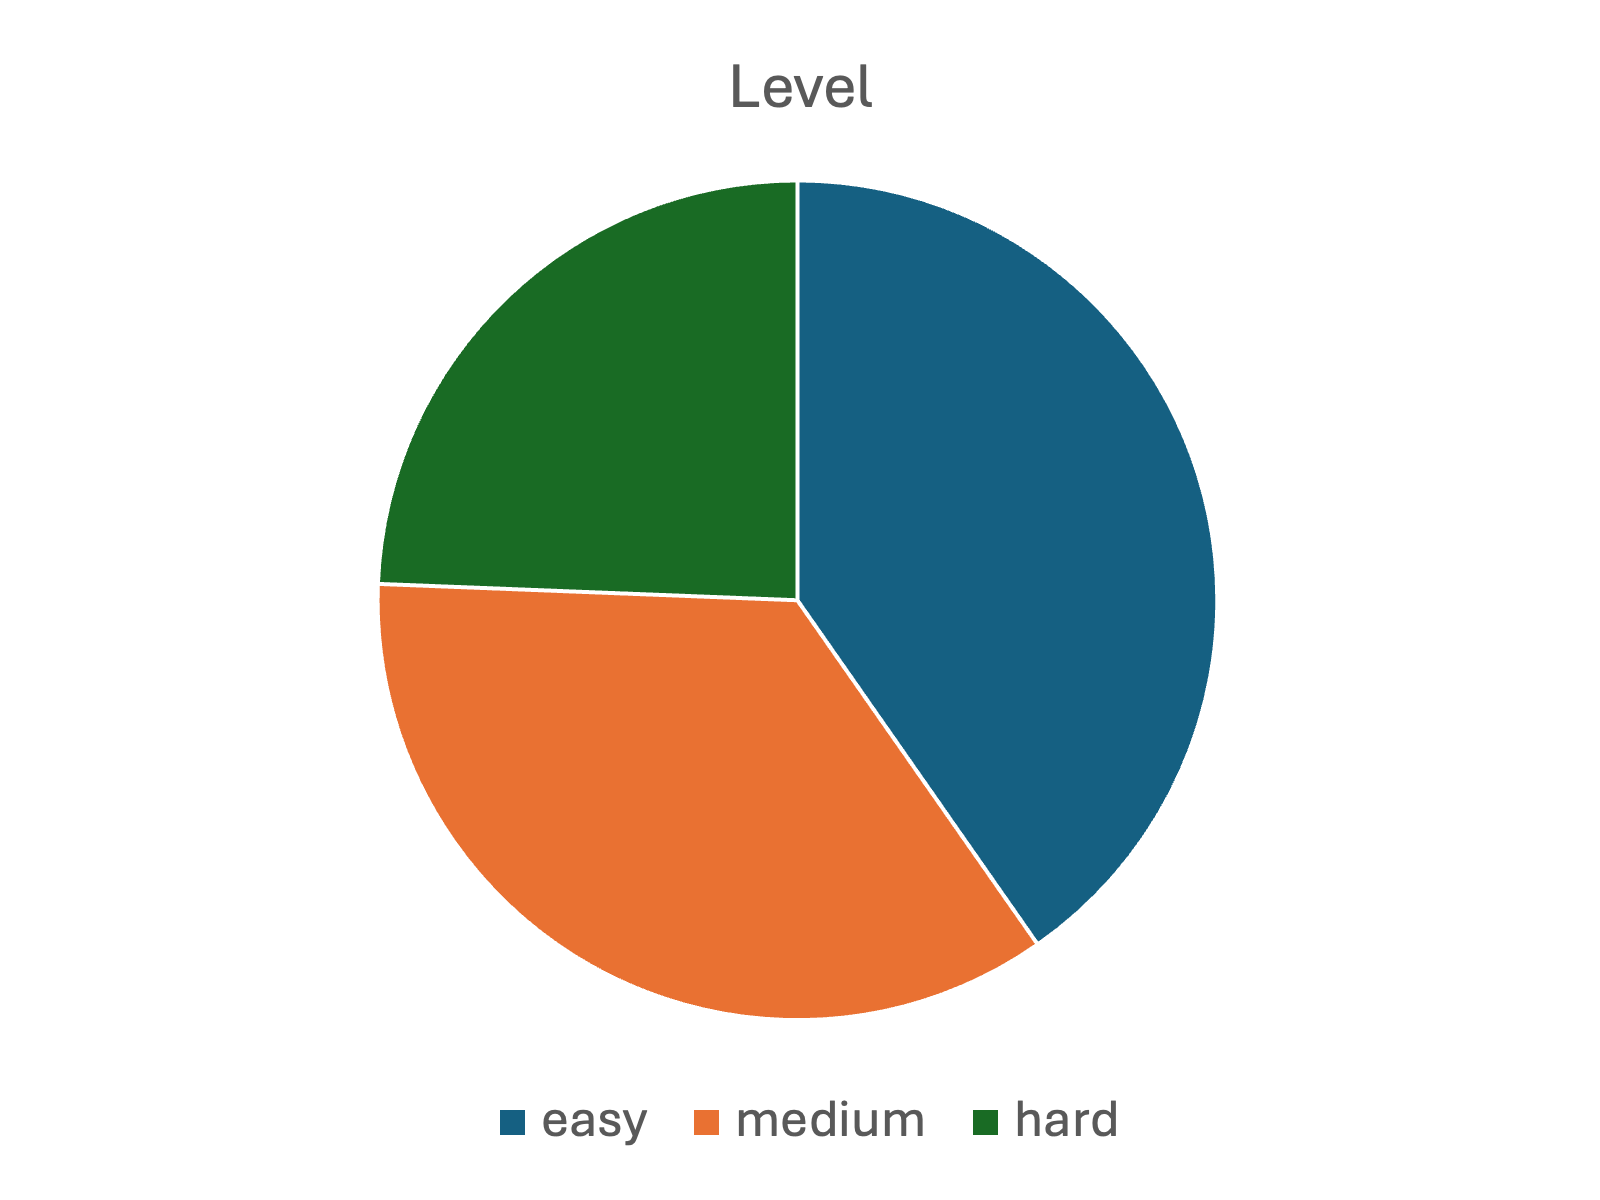
\includegraphics[width=0.8\textwidth]{images/dist_level.png}
%     \end{subfigure}
%     \caption{Distribution of tasks in A3. The above subfigure is the distribution by categories and the bottom subfigure is the distribution by difficulty levels.}
%     \label{fig:distribution}
% \end{figure}



Unlike existing approaches, A3 incorporates over 200 tasks derived from 20 widely used third-party applications, thereby significantly broadening the scope and variety of real-world scenarios. Each task is deliberately chosen to represent the most common functionalities and use cases of a given application. Moreover, every task is distinct, minimizing the repetition of actions and intentions. To better characterize the types of tasks included, we classify them into three categories: (i) operation tasks, (ii) single-frame query tasks, and (iii) multi-frame query tasks.

\textbf{Operation} tasks involve completing an action sequence on the device. For example, the instruction ``\textit{Search for ‘Taylor Swift’ on YouTube Music and subscribe}'' requires the agent to execute a specific action sequence. Such tasks are common in daily life, such as setting a reminder or playing music.

\textbf{Single-frame query} tasks prompt the agent to return a piece of information after completing the requested actions. For instance, given the instruction ``\textit{Search for stays in Beijing from Dec 27 to Dec 28, sort them by price from low to high, and provide the lowest price},'' the agent must identify the lowest price on the final state and present it as the answer. These tasks mirror common real-world queries, such as finding a restaurant’s contact information or a hotel’s nightly rate.

\textbf{Multi-frame query} tasks are more complex, requiring the agent to gather and process information across multiple steps before responding. For example, the task ``\textit{Search for a one-night stay in a one-bed room at Hilton Garden Inn Hong Kong for next week. Identify the cheapest day and its corresponding price}'' demands that the agent aggregate data from several days, compare prices, and then select the optimal result. Unlike single-frame queries, multi-frame tasks require the agent to retain and manipulate information across multiple interactions, rather than relying solely on the final state.

We divide all tasks into three tiers of difficulty. Tasks that a human can complete in five or fewer steps are considered easy, and those achievable in ten or fewer steps are deemed medium. All remaining operation tasks are classified as hard. Table~\ref{tab:distribution} illustrates the distribution of tasks in A3. Due to the fact that multi-frame query tasks are extremely hard for existing agents, we devote more effort in operation and single-frame query tasks for better evaluation of agents' capabilities. Moreover, task instructions related to dates are dynamically generated to ensure the date can be selected, such as in a hotel booking app.


\subsection{Evaluation}

In A3, we present two evaluation methods: (i) a task-specific evaluation function and (ii) a commercial LLM evaluation system. These methods operate independently and can be chosen by users, with the first focusing on predefined tasks and the second offering a scalable solution for adding tasks across various apps. And to mimic the real-world scenario, all tasks are evaluated by real-time states, which means all the contents are real-time, not predefined offline contents.

\subsubsection{Evaluation Function}
\label{sec:func-eval}

For over 200 tasks, we pair each task with a corresponding evaluation function. This function is used to assess whether the agent successfully completes the given task through various methods. Since each task involves different actions and goals, the evaluation criteria vary accordingly. The evaluation methods can be broadly categorized into two types:

\begin{itemize}[leftmargin=2mm]
    \item Element matching is the most commonly used evaluation method. It involves identifying key elements in an XML tree and comparing their attributes with ground-truth values. For instance, consider the task: ``Open Downloads in Coursera and tell me how much storage is used.'' In this case, the final state XML should contain an element that displays the total storage used by the app. The ground-truth value can be extracted by parsing the XML tree and then compared to the agent's response. In more complex scenarios, multiple elements may need to be retrieved, and several conditions must be met to determine if the agent's answer is correct. Additionally, when the XML data is insufficient, OCR (Optical Character Recognition) is used to extract text attributes directly from an element, serving as a substitute for XML parsing.
    \item Action matching is used when evaluation requires verifying specific positions. For example, in the task: ``Search for a flashlight on the Wish app, filter results by price under 100, then select the first item and add it to the wishlist,'' the agent must click on the first item displayed in the search results. Action matching ensures that the click coordinates fall within the bounding box of the first item.
\end{itemize}

The primary limitation of function evaluation arises from the conditions and rules defined within the function itself. This is because it is challenging for coders to account for all possible corner cases and avoid imposing overly strict conditions on action history or state elements when determining whether a task has been successfully completed. For example, if an agent navigates to an incorrect page but eventually returns to the correct state after a few steps, it becomes difficult for coders to establish appropriate conditions to accurately handle such scenarios. Another example is that after completing a task, a pop-up window may appear and obscure critical elements on the screen, leading the evaluation function to misjudge the outcome.


\subsubsection{LLM Evaluation System}
\label{sec:llm-eval}

\begin{table}
    \centering
    \begin{tabular}{l c}
    \toprule
        LLM & Eval Correct \\
        \midrule
        GPT-4o-2024-11-20 & 86\% \\
        Gemini-1.5-Pro & 80\% \\
        Claude-3.5-sonnet & 82\% \\
        \bottomrule
    \end{tabular}
    \caption{The correctness of LLM evaluation by human validation from 50 tasks. ``Eval Correct'' represents the correctness of LLM evaluation results determined by human.}
    \label{tab:gpt-gemini-eval}
\end{table}

\begin{table*}[ht]
    \centering
    \resizebox{0.9\linewidth}{!}{
    \begin{tabular}{l | c | c c c | c c c | c c}
        \toprule
        Agent / Model & Metric & Easy & Med. & Hard & Op. & S. Q. & M. Q. & Overall & V.S. Human \\
        \midrule \midrule
        \multirow{3}{*}{InternVL2-8B} & Func SR & 21.3 & 1.3 & 0 & 14.0 & 2.0 & 0.0 & 10.5 & 94.0 \\
        & LLM SR & 22.3 & 5.2 & 0.0 & 16.1 & 4.1 & 0.0 & 12.4 & 94.5 \\
        & ESAR & 32.2 & 20.3 & 20.5 & 31.8 & 19.7 & 21.2 & 26.9 & - \\
        \midrule
        \multirow{3}{*}{Qwen2.5-VL-7B} & Func SR & 23.4 & 5.2 & 0.0 & 17.5 & 0.0 & 0.0 & 12.9 & 94.0 \\
        & LLM SR & 27.7 & 7.8 & 0.0 & 19.6 & 8.2 & 0.0 & 15.9 & 93.5 \\
        & ESAR & 39.8 & 27.2 & 29.4 & 36.4 & 25.6 & 28.3 & 33.2 & - \\
        \midrule
        \multirow{3}{*}{UI-TARS-7B-SFT} & Func SR & 28.7 & 9.1 & 0.0 & 21.0 & 0.0 & 0.0 & 16.9 & 93.0 \\
        & LLM SR & 34.0 & 15.6 & 0.0 & 23.8 & 16.3 & 0.0 & 21.9 & 93.0 \\
        & ESAR & 55.8 & 40.1 & 41.8 & 51.1 & 36.2 & 35.7 & 46.5 & - \\
        \midrule \midrule
        \multirow{3}{*}{GPT-4o-2024-11-20} & Func SR & 5.3 & 0.0 & 0.0 & 3.5 & 2.0 & 0.0 & 2.5 & 96.0 \\
        & LLM SR & 8.5 & 0.0 & 0.0 & 4.9 & 2.0 & 0.0 & 3.9 & 95.5 \\
        & ESAR & 14.6 & 9.2 & 8.6 & 15.1 & 7.2 & 7.7 & 9.1 & - \\
        \midrule
        \multirow{3}{*}{Claude-3.5-sonnet} & Func SR & 11.7 & 2.6 & 0.0 & 8.4 & 2.0 & 0.0 & 6.5 & 94.0 \\
        & LLM SR & 13.8 & 2.6 & 0.0 & 9.8 & 2.0 & 0.0 & 8.8 & 93.9 \\
        & ESAR & 23.6 & 16.7 & 14.2 & 22.1 & 14.7 & 14.9 & 17.6 & - \\
        \midrule
        \multirow{3}{*}{AppAgent} & Func SR & 19.1 & 2.6 & 0.0 & 12.6 & 4.1 & 0.0 & 9.9 & 94.0 \\
        & LLM SR & 21.3 & 5.2 & 0.0 & 14.7 & 6.1 & 0.0 & 14.0 & 93.5 \\
        & ESAR & 26.7 & 20.5 & 18.6 & 27.1 & 21.7 & 16.8 & 23.8 & - \\
        \bottomrule
    \end{tabular}
    }
    \caption{The evaluation results in A3. The top three rows are GUI-finetuned or pretrained agents. The bottom three rows are or utilize commercial generalist LLMs. ``Func SR'' stands for task success rate by evaluation function. ``LLM SR'' stands for task success rate by commvercial LLM evaluation. ``EASR'' stands for essential state achieved rate. }
    \label{tab:eval_results}
\end{table*}

During the development of A3, we encountered similar challenges discussed above. Each task requires a unique evaluation function, which must be meticulously designed by coding experts with the ability to parse XML and define precise success conditions. However, even experienced developers may struggle to account for all possible scenarios. This reliance on manual coding and condition setting significantly slows down the creation of evaluation functions. To overcome these limitations, we propose a commercial LLM-based evaluation system that harnesses the advanced capabilities of large language models (LLMs), such as GPT, Gemini, and Claude, to enable fully autonomous task evaluation.

LLM evaluation system can be categorized into three methods, which are (i) final state evaluation, (ii) sequence state evaluation and (iii) essential state evaluation.

\begin{itemize}[leftmargin=2mm]
\item Final state evaluation is conducted by LLM evaluators, who assess whether a task has been successfully completed based solely on the final execution state. This approach enables quick and accurate evaluation for tasks where the final state provides all the necessary information for judgment, such as ``Open the notification page of CNN.'' In those cases, the final state fully encapsulates the task requirements. However, this method can result in misjudgments if the final state changes unexpectedly or fails to include the information needed for evaluation.
\item Sequence state evaluation is designed to overcome the limitations of final state evaluation by assessing task completeness using a combined sequence of all states throughout the execution. In this approach, all screenshots are merged into a single image, and the corresponding XMLs are serialized. This method provides accurate and efficient evaluation for simpler tasks where the sequence length is fewer than six states. However, for longer sequences, the combined image becomes overly compressed and flat, leading to potential confusion and hallucination during evaluation.
\item Essential state evaluation offers the most comprehensive approach among the three evaluation methods. In this method, each task is broken down into a series of ``essential states.'' For example, the task ``Open Gmail and select the 'Draft' folder'' can be divided into two essential states: [``Gmail is opened,'' ``Draft folder is selected'']. A sliding window is then applied to the entire sequence, grouping a set of states and XMLs, similar to sequence state evaluation. However, instead of evaluating the entire sequence, evaluators determine which essential states are achieved within the sliding window. The window moves incrementally from the start to the final state, and evaluators collect all the essential states that have been achieved. If the set of achieved essential states matches the complete list of essential states, the task is confidently deemed successful. This method also introduces an additional evaluation metric, the \textbf{E}ssential \textbf{S}tate \textbf{A}chieved \textbf{R}ate (ESAR), which is calculated as the number of achieved essential states divided by the total number of essential states. ESAR provides a more granular performance assessment for agents. For example, even if a task fails, an agent that achieves 2 out of 3 essential states performs better than one that achieves only 1 essential state. More detailed essential states generation is in Appendix~\ref{app:essential-states}
\end{itemize}


Hallucination is an inherent limitation of LLMs, leading to occasional misjudgments even in the most advanced commercial models. However, evaluator voting can significantly reduce the rate of misjudgment. We conducted experiments using three of the most advanced commercial LLMs, comparing their evaluations against human judgment on 50 tasks. The accuracy results are presented in Table~\ref{tab:gpt-gemini-eval}. When evaluator voting is applied, the accuracy of the judgments increases to a conservative estimate of over 92\%, demonstrating a high level of confidence in the evaluation outcomes.


\section{Experiments}

% \begin{table}
%     \centering
%     \begin{tabular}{c c c}
%         \toprule
%         Test Subset & Test Level & Succ. Rate \\
%         \midrule
%         \multirow{2}{*}{IDD} & High & 69.6 \\
%         & Low & 92.1 \\
%         \midrule

%         Category & High & 51.8 \\
%         Unseen & Low & 84.4 \\
%         \midrule

%         App & High & 56.8 \\
%         Unseen & Low & 83.0 \\
%         \midrule

%         Task & High & 73.7 \\
%         Unseen & Low & 88.5 \\
%         \bottomrule
%     \end{tabular}
%     \caption{Static frame evaluation results on \textsc{AndroidControl} test set.}
%     \label{tab:android-control-exp}
% \end{table}





\subsection{Evaluation}

We evaluate six models or agents and compare their performance using the A3 evaluation system. Three of these models (InternVL2~\citep{chen2024internvl}, Qwen-2.5-VL~\citep{Qwen2.5-VL}, UI-TARS~\citep{qin2025ui-tars}) are fine-tuned or pre-trained specifically for GUI tasks, while the other three (GPT-4o-2024-11-20, Claude-3.5-sonnet, AppAgent~\citep{yang2023appagent}) are commercial LLMs or models that leverage commercial LLMs.

We select the 7B versions of Qwen2.5-VL and UI-TARS, along with the 8B version of InternVL2, to ensure a comparable agent size. Qwen2.5-VL is a generalist Multimodal Large Language Model (MLLM) pre-trained on GUI-related data, while UI-TARS further fine-tunes Qwen2-VL on GUI-related data with enhancements for reasoning and screen understanding. Both agents are evaluated following their official inference guidelines. Additionally, we apply supervised fine-tuning to InternVL2 on AMEX ~\citep{chai2024amex} and \textsc{AndroidControl}~\citep{li2024androidcontrol} datasets to serve as a baseline agent (further fine-tuning details are provided in Appendix~\ref{app:finetune}). For GPT-4o, we incorporate Set-of-Mark (SOM)~\citep{yang2023set} to improve element recognition and selection, while for Claude, we adapt a specialized prompt modified from the ``Claude-computer-use'' prompt to better suit mobile scenarios. AppAgent is used directly without any modifications.

Table~\ref{tab:eval_results} presents the main evaluation results for the six agents. ``Func SR'' refers to the task success rate as evaluated by predefined functions, ``LLM SR'' represents the task success rate as assessed by commercial LLMs, and ``ESAR'' stands for the essential states achieved rate.

The table reveals that agents pre-trained or fine-tuned on GUI tasks generally outperform generalist models, suggesting that commercial generalist models lack sufficient adaptation for GUI-specific tasks. Even though Claude’s ``computer use'' model demonstrates significantly better performance than GPT-4o, it still faces a substantial domain gap between desktop environments and mobile scenarios. AppAgent, on the other hand, leverages GPT-4o’s basic image understanding capabilities and incorporates additional exploration and indexing techniques, resulting in a significant performance improvement compared to the original GPT-4o and Claude’s ``computer use'' model. Moreover, UI-TARS achieves considerably higher success rates than Qwen2.5-VL, underscoring the value of task-specific fine-tuning and the impact of reasoning data. Finally, InternVL2, as a baseline fine-tuned agent, demonstrates that even with minimal fine-tuning, smaller models can outperform well-designed commercial LLMs on GUI-specific tasks.

We observe that commercial LLM evaluations consistently yield higher success rates (SRs) compared to function-based evaluations. Upon analyzing their evaluation processes, we find that LLMs apply looser criteria than functions which often enforce strict conditions, such as requiring a specific final state or a predefined sequence of actions. In contrast, commercial LLM evaluations align more closely with human judgment, as they assess tasks based on essential states and the overall sequence of actions. Additionally, the ESAR metric offers a more detailed evaluation, even when the task success rate is all 0.0 for difficult tasks. ESAR reflects an agent's ability to break down complex tasks into simpler essential states, with higher ESAR values indicating better performance. This trend aligns with the patterns observed in task SRs.

We further validate the function-based and commercial LLM evaluation results through human observation. The average accuracy of commercial LLM evaluations is approximately 93\%, closely matching the estimate calculated in Section~\ref{sec:llm-eval}. This high level of accuracy, confirmed by human validation, strongly supports the reliability of commercial LLM evaluations in real-world scenarios. Additionally, the observation that LLM evaluations are occasionally more accurate than function-based evaluations can be attributed to the reasons outlined in Section~\ref{sec:func-eval}.


\subsection{Error Case Analysis}

To better demonstrate the obstacles that agents encounter in the real-world scenario, we provide some most common error cases during the observation of the evaluation.

\begin{itemize}[leftmargin=5mm]
    \item Perform \texttt{CLICK} at wrong coordinate. If the coordinate is wrong, either the screen doesn't change (click at nothing), or it goes to a wrong state, which requires self-correct ability to get back on the track. This type of errors is mainly due to the insensibility of LLMs to digits.
    \item Wrong action planning. This happens when an agent predicts completely wrong action type. With reasoning and thinking, UI-TARS still suffers from the action prediction when a task is complex.
    \item Start typing before the element is selected. We see many cases where the agent starts to type text when the search bar or other element is not clicked or selected. This is possibly due to the inconsistent annotation style in the existing datasets: sometime annotators click the element before typing while sometime they don't if the element is automatically selected.
    \item ``Stop'' issue. Some agents such as Qwen2.5-VL often stops too early and other agents such as UI-TARS fail to stop even if the task is finished successfully.
\end{itemize}


\section{Discussion}

\begin{itemize}[leftmargin=5mm]
    \item The integrated tasks and evaluation functions are defined on specific versions of apps, which may lead to different evaluation results on different app versions.
    \item All datasets are used consistently with the licenses, such as Apache 2.0 of both \textsc{AndroidControl} and AMEX.
    \item No existing potential risk is shown during the evaluation.
\end{itemize}

\section{Conclusion}

We introduce Android Agent Arena (A3), a comprehensive and autonomous online evaluation system for GUI agents. A3 incorporates both human-validated task-evaluation pairs and an autonomous LLM-based cross-validation process. The tasks span a wider range of categories and applications, enabling the evaluation of agents' capabilities in both operation execution and information retrieval across three levels of difficulty. The autonomous evaluation process significantly minimizes human intervention and workload, offering a more efficient approach to scaling the number of evaluation tasks.




% Bibliography entries for the entire Anthology, followed by custom entries
%\bibliography{anthology,custom}
% Custom bibliography entries only
\bibliography{custom}

\appendix

\section{Appendix}

For anonymization, the url is temporarily at \url{https://anonymous.4open.science/r/AVD-Control-Evaluation-F758}.

\subsection{App Selection}
\label{app:app-selection}

We select the apps from different categories in Google Play Store, where only two categories (News and Shopping) contains 2 apps. Those apps satisfy two conditions: (i) can be installed and run normally on any emulators; (ii) in top 15 list of the category. The first condition is to ensure the apps can run on any devices, because many apps don't support x86 platforms. The second condition ensures the popularity of the apps to represent the daily scenario.

\subsection{Task Generation and Examples}
\label{app:task-gen-eg}

The tasks are all created by system designers and function coder. Each coder is in charge of an app and creates its most common usages and tasks based on the app functions. For example, tasks of shopping apps will contain essential states such as ``search for products'', ``add to wishlist'', ``add to cart'', ``sort by price'', etc. The difficulty of tasks can be controlled by different number of essential states. For example, ``sort by price'' or ``filter to under \$100'' can be optional to modify the task difficulty level. Coders are also required to keep the ratio of three levels at around 5:3:2. Then the coder will determine the level of the task by executing a ``Gound Truth'' trace and saving all the information such as screenshot, XML and action history. These information are used to design the evaluation functions. The functions are then validated by three correct traces and three wrong traces.

The following are task examples:

\paragraph{Easy}

\begin{itemize}[leftmargin=5mm]
    \item Open Yelp and search for pizza nearby.
    \item Search for 'Micheal Jackson' on YouTube.
\end{itemize}

\paragraph{Medium}

\begin{itemize}[leftmargin=5mm]
    \item Is the book 'Romeo and Juliet' in my wishlist on Wish?
    \item Go to 'Taylor Swift' page and subscribe on YouTube Music.
\end{itemize}

\paragraph{Hard}

\begin{itemize}[leftmargin=5mm]
    \item Open Booking.com and search for stays in Beijing from Nov 27 to Nov 28. Then sort by price from low to high, and tell me the lowest price.
    \item After sorting the results by distance for nearby BBQ on Google Maps, select the first store, and start navigation.
\end{itemize}

\subsection{Essential States}
\label{app:essential-states}

The essential states of a task can be generated by two approaches: (i) human definition and (ii) LLM generation (GPT-4o-2024-11-20). To ensure the correctness and precision, users can choose the human definition. For example, if the task is ``Open Booking.com and search for one-way flight from Beijing to Shanghai on Feb 20. Select two adults.'' The user can define the essential states: ["Device is in Booking.com app", "One-way flight is selected", "Departure city is set to Beijing", "Arrival city is set to Shanghai", "Departure date is set to Feb 20",  "Number of adults is set to 2", "Search results are displayed"]. To autonomously execute the evaluation process, users can choose LLM generation.  We also validate the LLM generated essential states of 30 tasks, 10 for each difficulty level. The validation result is that the correctness of LLM generated essential states reaches 100\%, which means it can perfectly split a task into essential states as humans do. The prompt is as followed:

\begin{lstlisting}[style=prompt, caption={Prompt for essential states generation.}]
You are given a task instruction, which a user wants to perform on a mobile device.\n
The task is: {task}\n
The task can be splited by a sequence of essential states, which means the states that are necessary to achieve the task.\n
For example, if the task is "Open Booking.com and search for one-way flight from Beijing to Shanghai on Feb 20. Select two adults." the essential states are: ["Device is in Booking.com app", "One-way flight is selected", "Departure city is set to Beijing", "Arrival city is set to Shanghai", "Departure date is set to Feb 20",  "Number of adults is set to 2", "Search results are displayed"]\n
Now please provide the essential states to achieve the task. Do not include trivial states like "Device is in Home page" or "Device is unlocked". Only include the states that are necessary to achieve the task.\n
\end{lstlisting}



\subsection{Prompts}

The simplified prompt for GPT-4o to evaluate essential states (Section~\ref{sec:llm-eval}) is as followed:

\begin{lstlisting}[style=prompt, caption={Prompt for essential states evaluation.}]
Given a list of UI elements, an image consisting of screenshots
and a list of states, judge whether one or more states are correctly
achieved in the conbimed screenshots. \n
The sequence of states is: {states_str} \n
The sequence of UI elements corresponding to the screenshots are: {elements} \n
You are also provided with an answer to the final question: {answer} \n
\n
You are required to reply with the states that are correctly achieved
without any changes. If none of the states are correctly achieved, 
reply with "none". \n
If the "answer" is correct, reply with the the "answer" attribute "yes" and 
otherwise "no". \n
Also provide the reason for your answer.
\end{lstlisting}


The simplified prompt for GPT-4o to directly evaluate the task performance is as followed:

\begin{lstlisting}[style=prompt, caption={Prompt for final state evaluation.}]
GGiven a task, a screenshot image and a json file of the final screen, judge whether the task is completed correctly. \n
The task is '{task}'. And here is the json file which contains elements corresponding to the marks on the screenshot: {xml}.\n
To correctly judge the performance, you should consider element states such as 'selected' and 'activated' to check whether specific condition is satisfied. You also need to consider the content-desc attributes of elements to check the result correctness. \n
Answer with only "yes" or "no". The reason should consider the conflicting elements or wrong states
\end{lstlisting}

\subsection{Finetuned Agent}
\label{app:finetune}

We use the 8B model of InternVL2 as the base model. We train the model on 8 A100 GPU for 27 hours on \textsc{AndroidControl} and AMEX, following the default finetuning settings. 
The data is directly used for supervised finetuning, such as ``Given the task: xxxxx, your action history: xxxxx, predict next action on the screen <image>'' and ``CLICK<coor>100, 100</coor>''.

\subsection{Demonstrations}

Here we provide some demonstrations of errors during evaluation (See Figure~\ref{fig:demo-1} and Figure~\ref{fig:demo-2}). We can see that the agent predicts several steps correctly but if one action is wrong, the agent would fail the task. 

\begin{figure*}
    \centering
    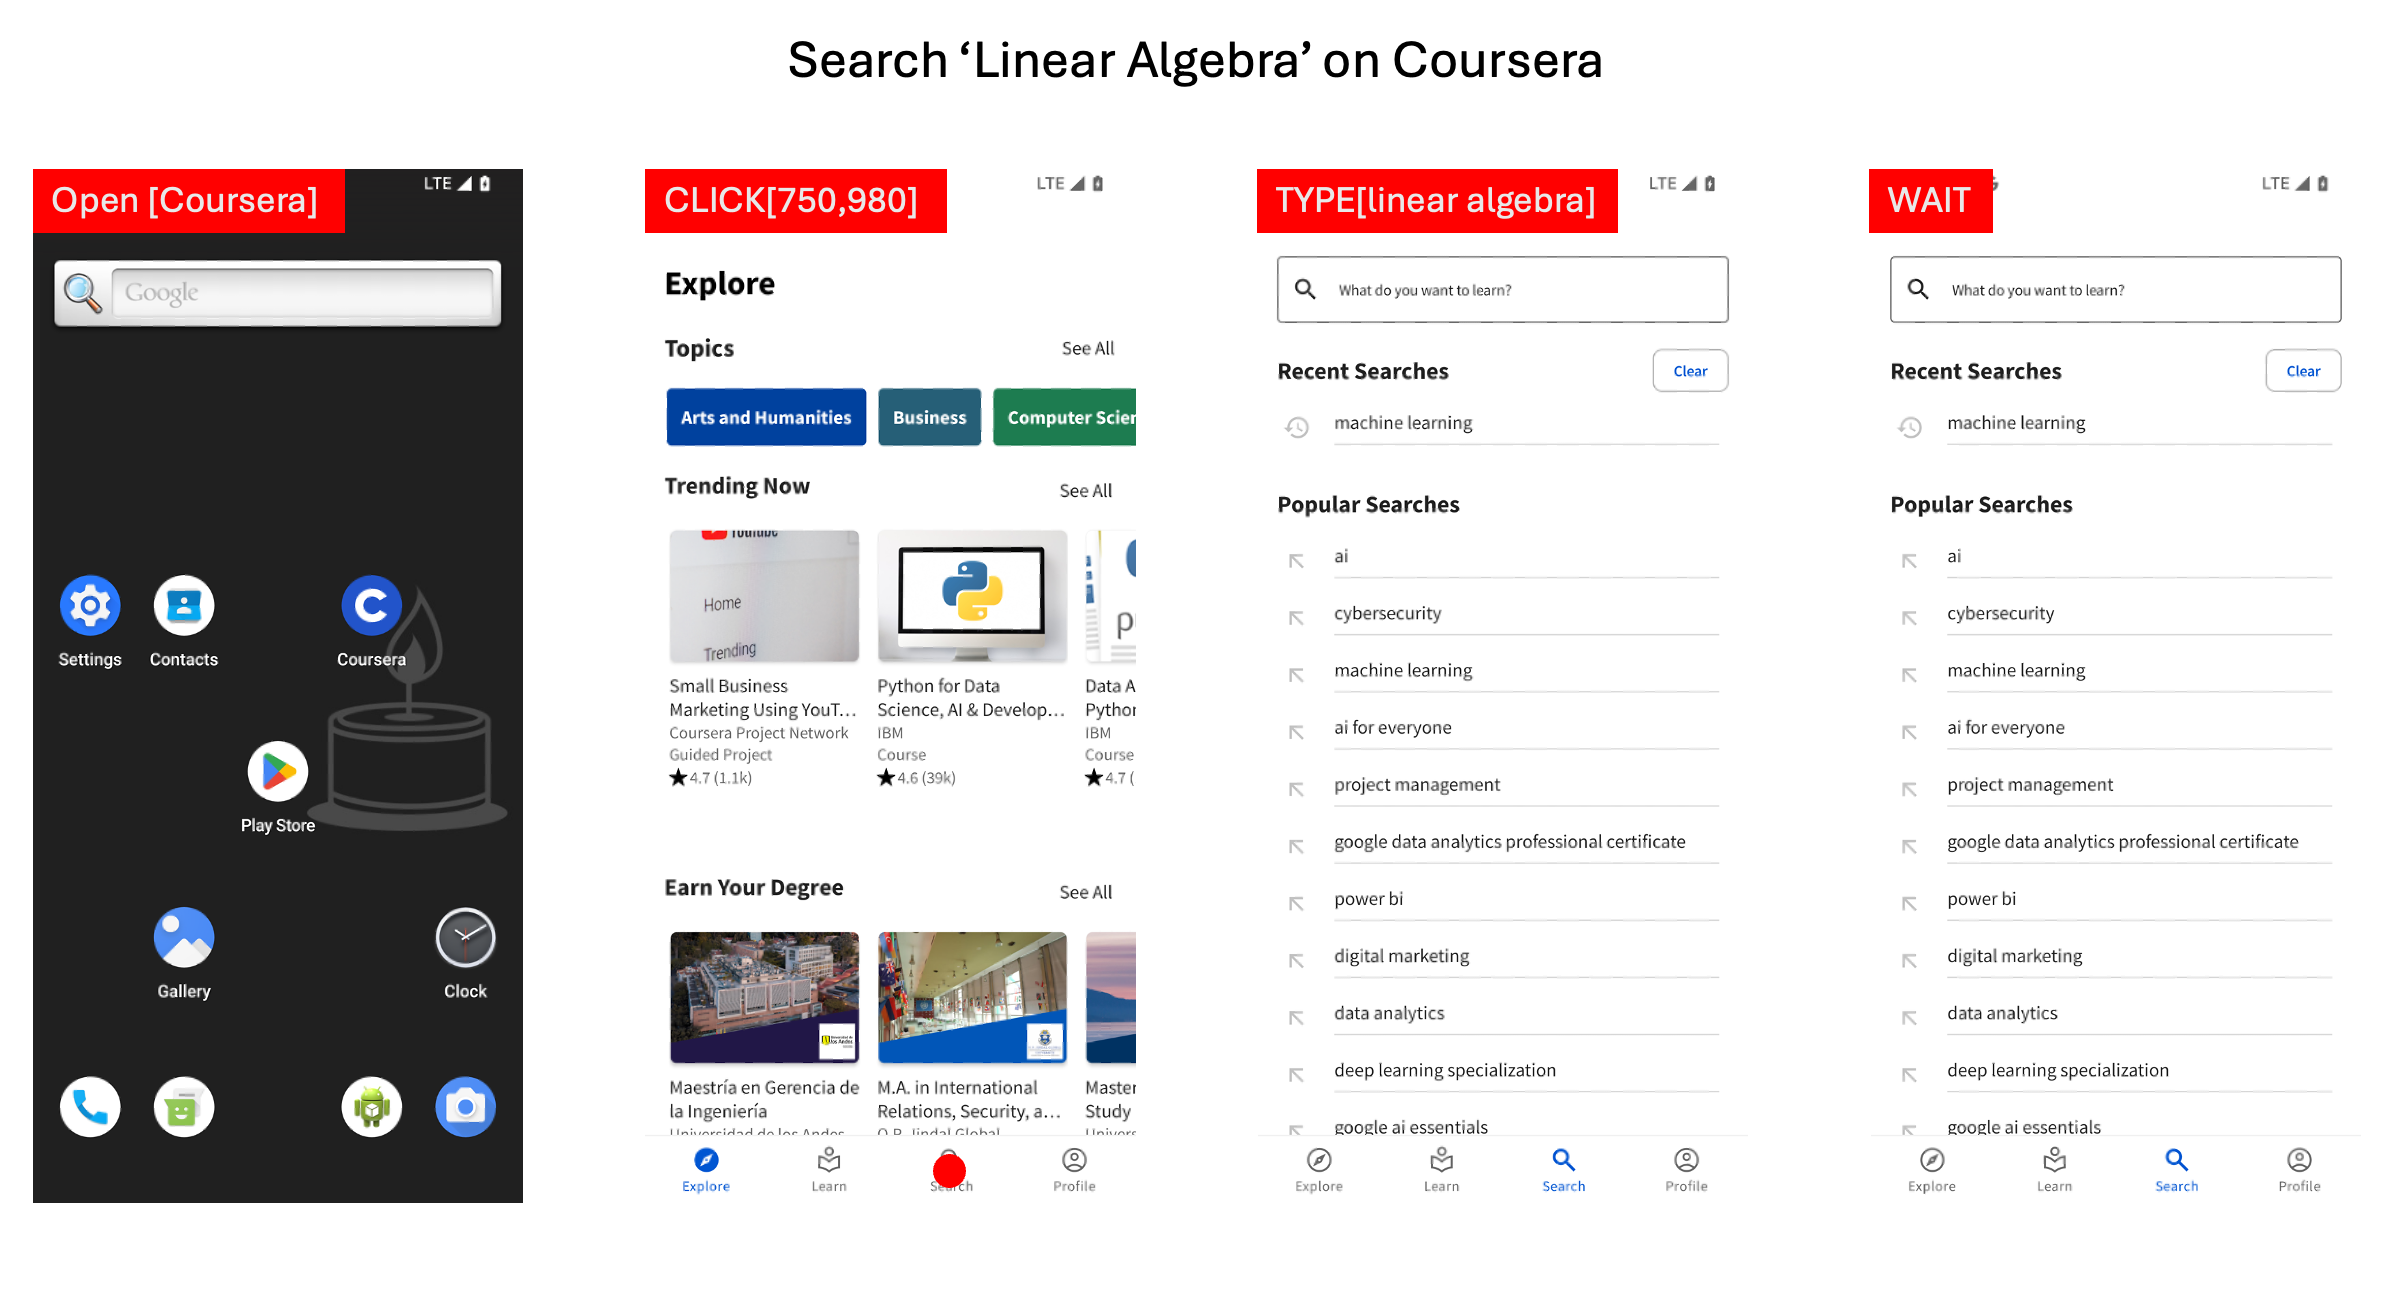
\includegraphics[width=0.97\linewidth]{images/demo-1.png}
    \caption{Step 1 and Step 2 are correct, however, the agent starts typing before the search bar is clicked or selected, so the process sticks at this situation and the agent keeps typing and waiting.}
    \label{fig:demo-1}
\end{figure*}

\begin{figure*}
    \centering
    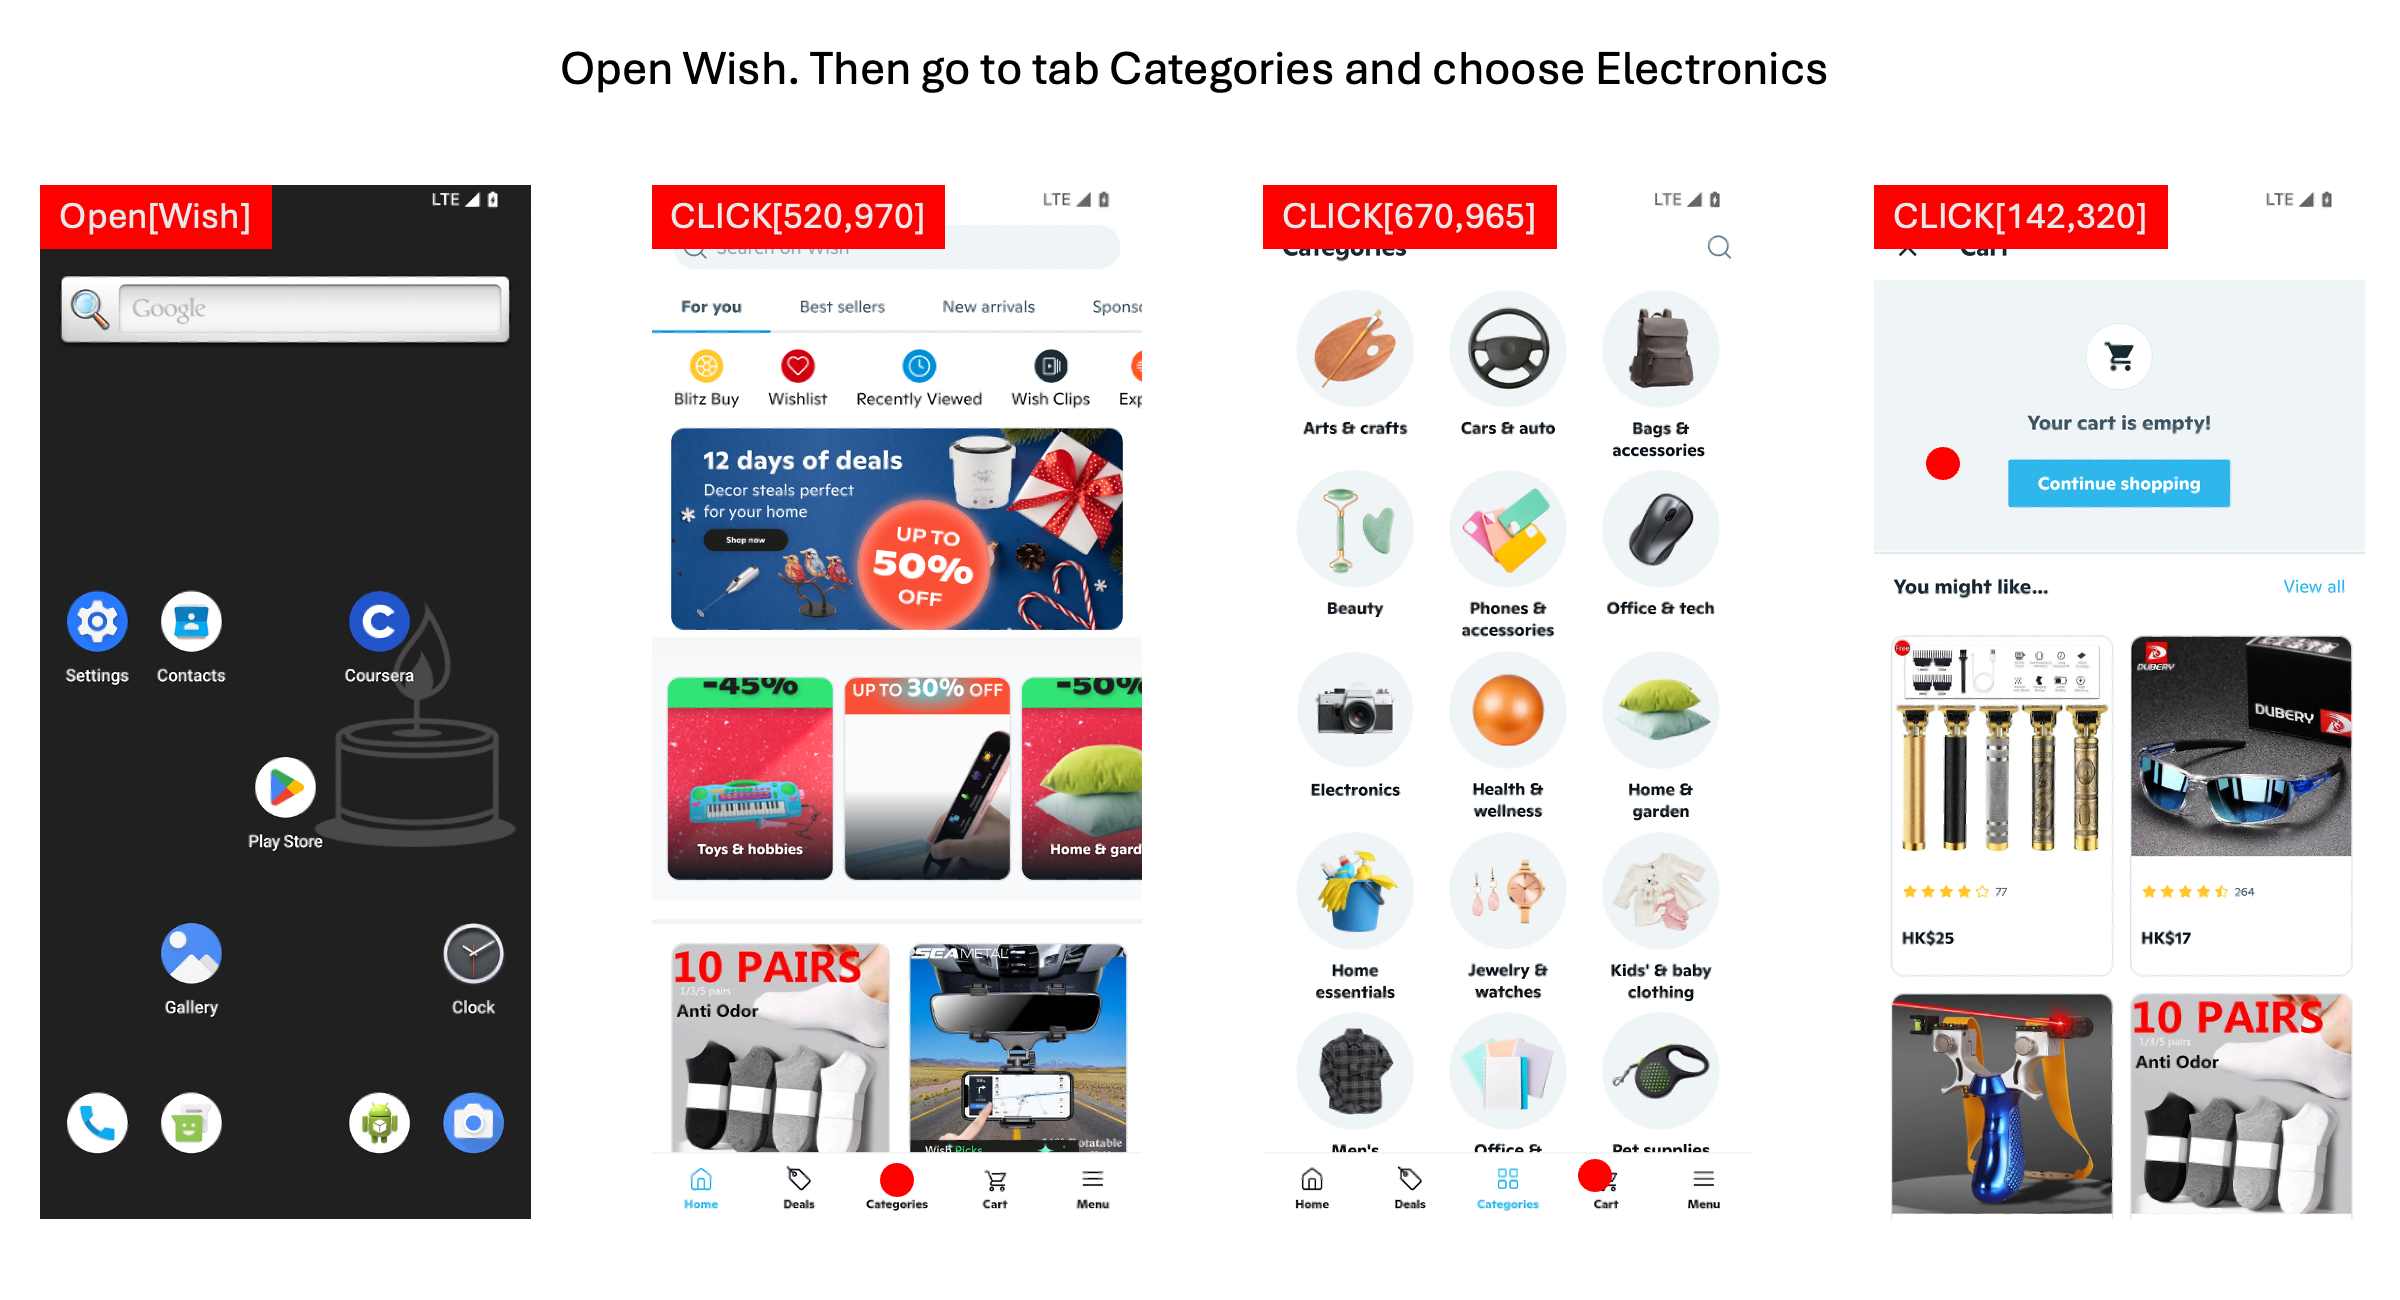
\includegraphics[width=0.97\linewidth]{images/demo-2.png}
    \caption{Step 1 and Step 2 are correct, however, the agent predicts a wrong click coordinate and accidentally go to the shopping cart. It should go back but seems it lacks the capability to do that and gets stuck in the shopping cart.}
    \label{fig:demo-2}
\end{figure*}


\end{document}
